I have been working with robot manipulators for quite a while now. One of the things that has surprised me most about robots is their almost unbelievable incompetence. Popular science fiction led me to believe that robots would have superhuman abilities. 

To be fair, many robots \textit{really are} superhuman. Just look at any factory floor. These days, factories (especially car factories) are filled with huge, lumbering industrial robots that do the same tasks again and again at breakneck speeds -- welding, lifting huge loads, bending metal, and precisely placing tiny parts. That's something I couldn't do with my measly human hands and brain even in principle.

But in spite of their obvious advantages, industrial robots have an embarassing secret: for the most part, they're programmed in an ad-hoc matter by hand, and follow their programming without question. You might notice that on the factory floor, the robots are in cages, and there aren't any people around. This is because when you've got a 4-ton robot moving around at breakneck speeds according to a rigid program, it doesn't play nicely with any human beings that might be standing in the way. You might also notice that in factories, each robot performs an extremely well-defined task (such as screwing in four specific bolts, or spraying paint at one specific part of a specific kind of car chassis). The sad matter of fact is, if the task that the industrial robot has to perform were to change only slightly, its program would fail spectacularly.

In undergrad, as part of a manipulation class we programmed an ABB industrial robot to pick highlighters out of a box in Matt Mason's lab, and show them to a camera. It was supposed to pick thousands of these things out of the bin to train a machine learning algorithm. The robot was using simple position control to move about. It would drop the markers on a styrofoam ramp, whcih would then slide back into the bin. At a rate of about one highlighter every twenty seconds, it would take many hours to train the system. While waiting for the robot to complete its task, I fell asleep on the couch in the lab. A couple of hours later, I was awoken by a loud \textit{crash}. Somehow, the robot had smashed the ramp to bits, and was presently dropping markers onto the floor as if nothing had happened. That's not exactly superhuman performance.

As you might guess, robots need to be a lot smarter to tackle real-world tasks, where things are constantly changing and you can't afford to be so rigid. That means taking in information from sensing, detecting failure, and coming up with new plans of action as tasks change. As humans, we take these things for granted. Even the youngest babies are capable of reacting to changes in their environments, and next to industrial robots look like geniuses when it comes to manipulating novel objects. Robotics research is all about making this kind of baby-like performance possible. The holy grail of robotic manipulation would be a system that could adapt as quickly as a newborn. This phenomenon (sometimes called \textit{Moravec's Paradox}, after Hans Moravec, the famous CMU roboticist) haunts robotics. Humans think manipulation is easy because we were quite literally born to manipulate. We are like natural-born piano virtuous who glibly declare that piano playing is easy, and all it takes is a bit of intuition.

I witnessed several other instances of robotic incompetence during the DARPA ARM-S challenge. The idea behind the challenge was that teams of manipulation experts from universities around the world would program a robot to autonomously complete some ``simple'' manipulation tasks such as picking up objects, using simple tools, opening doors, etc. I was lucky enough to work as a student intern and later as a software engineer on this multi-year project for the team at NREC. If I was to describe our team's initial strategy with one word, it would be \textit{modularity}. We broke the problem of grasping down into a few simple steps described in the literature as the ``grasping pipeline'' (\figref{fig:grasp_pipeline}).

\begin{figure}
\centering
	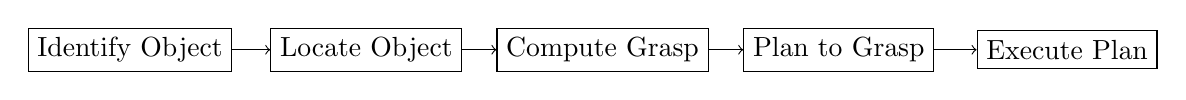
\begin{tikzpicture}
		\node[draw] (ident) at (0, 0) {Identify Object};
		\node[draw] (locate) at (3, 0) {Locate Object};
		\node[draw] (plan_grasp) at (6, 0) {Compute Grasp};
		\node[draw] (motion_plan) at (9, 0) {Plan to Grasp};
		\node[draw] (close) at (11.9, 0) {Execute Plan};
		\path [draw, ->] (ident) -- (locate);
		\path [draw, ->] (locate) -- (plan_grasp);
		\path [draw, ->] (plan_grasp) -- (motion_plan);
		\path [draw, ->] (motion_plan) -- (close);
	\end{tikzpicture}
\caption{The so-called grasping pipeline.}
\label{fig:grasp_pipeline}
\end{figure}

The idea behind the grasping pipeline is that the ``perception people'' can simply work on the first two steps (identifying and locating objects), the ``planning people'' can work on on the third and fourth steps (determining how to grasp a known object and how to exectue that grasp), and finally the ``controls people'' can focus on the final step, which is actually executing the plan that was passed to them. 

In this context, each module is just a black box with well-defined inputs and outputs. As specialists, we like such black boxes because they allow us to keep the messy bits of the other guy's box out of our mind and focus on solving the problem. The perception people never need to ask ``how will uncertainty in my perception system affect the grasp planner?'' the planning people never have to ask ``what if the execution fails?'' and the execution people never have to ask ``what do I do if the plan is wrong?''

Of course, when we strung all the black boxes together, we got a result that was less than satisfactory. Very often, the robot's beautiful grasp plan would put it a few millimeters away from where it was supposed to be, the fingers would close, and the grasp would fail completely. 

Why does this happen? In a word: \textit{uncertainty}. The perception system didn't know exactly where the objects were. The robot's model of its own kinematics were not exactly correct. The controller was noisy and didn't perfectly follow the planner's trajectory. Ultimately, the boxes were not supposed to be so black. The perception system should have detected that the robot wasn't where it was supposed to be, the planning system should have generated a new plan of action when this was detected, and the execution system should have responded to the new plans. In other words, \textit{Moravec's Paradox} had reared its ugly head in our system design, making it far too optimistically simple.

By the end of the challenge, our system design had changed to something much more complex and robust. The core of our design shifted from \textit{planning} to \textit{control}. We had a perception system that fed data directly into the controller, which directly adjusted according to changes in the environment. 

In my opinion, the critical bit of engineering that changed our grasping pipeline from something embarassing to something workable was 3D visual servoing. The idea behind 3D visual servoing is quite simple: you perceive the robot and its goal, figure out how much error there is between the current state of the robot and where you want it to be, and then you tell the controller to take a step toward reducing the error. This strategy has a beautiful simplicitly which naturally reduces uncertainty. Errors in the robot's kinematics, object sensing, and control are all forced into the same reference frame, where small corrections can be made to reduce them. 

This is far better than trying to correct all the error beforehand using calibration and then blindly trying to execute a plan with the faith that your calibration is perfect. In fact, our servoing allowed us to be lazy. We hardly ever recalibrated the robot's joint encoders or camera extrinsics -- the visual servoing made all of that unnecessary.

This thesis is about developing systems which use perception in the loop with a robot arm to correct error in its calibration. The first section is about work I did with ARM-S on tracking the robot arm with an external depth camera, which was a critical component in our visual servoing architecture. The second section takes the same idea and extends it to a hand-mounted depth camera which cannot see any part of the robot. This was done for the ADA project at the Personal Robotics Lab. The third section generalizes this idea to a SLAM framework which can support multiple sensor types, calibration parameters, and uncertainty models; which I developed while visiting the Dyson Robotics Lab at Imperial College London.

My hope is that the research I present here will help elucidate some of the challenges of properly calibrating and tracking robots online, and how some general techniques from computer vision and SLAM can be used for this purpose.